\section{Pipeline capacity algebra}\label{sec:pipeline-capacity-algebra}
\noindent The preceding section defines the notions of the capacity and transmission vector sets for single pipelines and functions respectively. This section will extend these notions to multi-pipeline networks and functions by defining a capacity algebra to calculate the joint capacity and transmission vector sets of composed pipelines and functions.

\para{Problem definition:} We define the problem of composing capacity and transmission vector sets as the vector set composition (VSC) problem: given a set of pipelines $P$ or functions $F$ and their associated vector sets $cvs(P)$ and $tvs(F)$, what is the $cvs$/$tvs$ of some composition of elements in that set?

\subsection{Pipeline capacity vector set algebra}
\para{Serial and parallel pipeline composition:} We begin developing our algebra by examining pipeline capacity vector set (cvs) composition. To start, we define two pipeline composition operations, which we term serial and parallel composition.

\vspace{3mm}
\noindent \textsc{Definition 1 - Serial composition:} Under serial composition, a given pipeline $p_1$ can transmit limited computation results to the following pipeline $p_2$ by writing a $w$ bit \textit{composition header} to outgoing packets at egress for $p_2$ to read.

\vspace{3mm}
\noindent \textsc{Definition 2 - Parallel composition:} Under parallel composition, a given pipeline $p_1$ can choose a destination pipeline from a set of possibilities $P$ to forwards a packet to for additional processing. We say that the pipelines $p_i$ in $P$ are composed in parallel, and that $p_1$ is composed in serial with $P$.

\para{Pipeline cvs composition operators:} We formalize our pipeline cvs algebra by introducing the notation $\times$ and $+$ to represent the cvs serial and parallel composition operators respectively. The $\times$ and $+$ operators take the cvs of two pipelines and return the cvs of the pipeline formed by composing the two original pipelines in serial and parallel respectively.

For example, serially composing the two pipelines $p_1$ and $p_2$ (\ie\ allowing $p_1$ to send traffic to $p_2$ for further processing), where pipeline $p_i$ has cvs $cvs_i$, produces a pipeline with cvs $cvs_1 \times cvs_2$ (Fig~\ref{fig:serial-and-parallel-composition}a.) Serially composing $p_1$ with the parallel composition of $p_2$ and $p_3$ (\ie\ allowing $p_1$ to send traffic to either $p_2$ or $p_3$ for further processing) produces a pipeline with cvs $cvs_1 \times (cvs_2 + cvs_3)$ (Fig~\ref{fig:serial-and-parallel-composition}b.).

\begin{figure}[tbh]
    \centering
    \vspace{-1mm}
    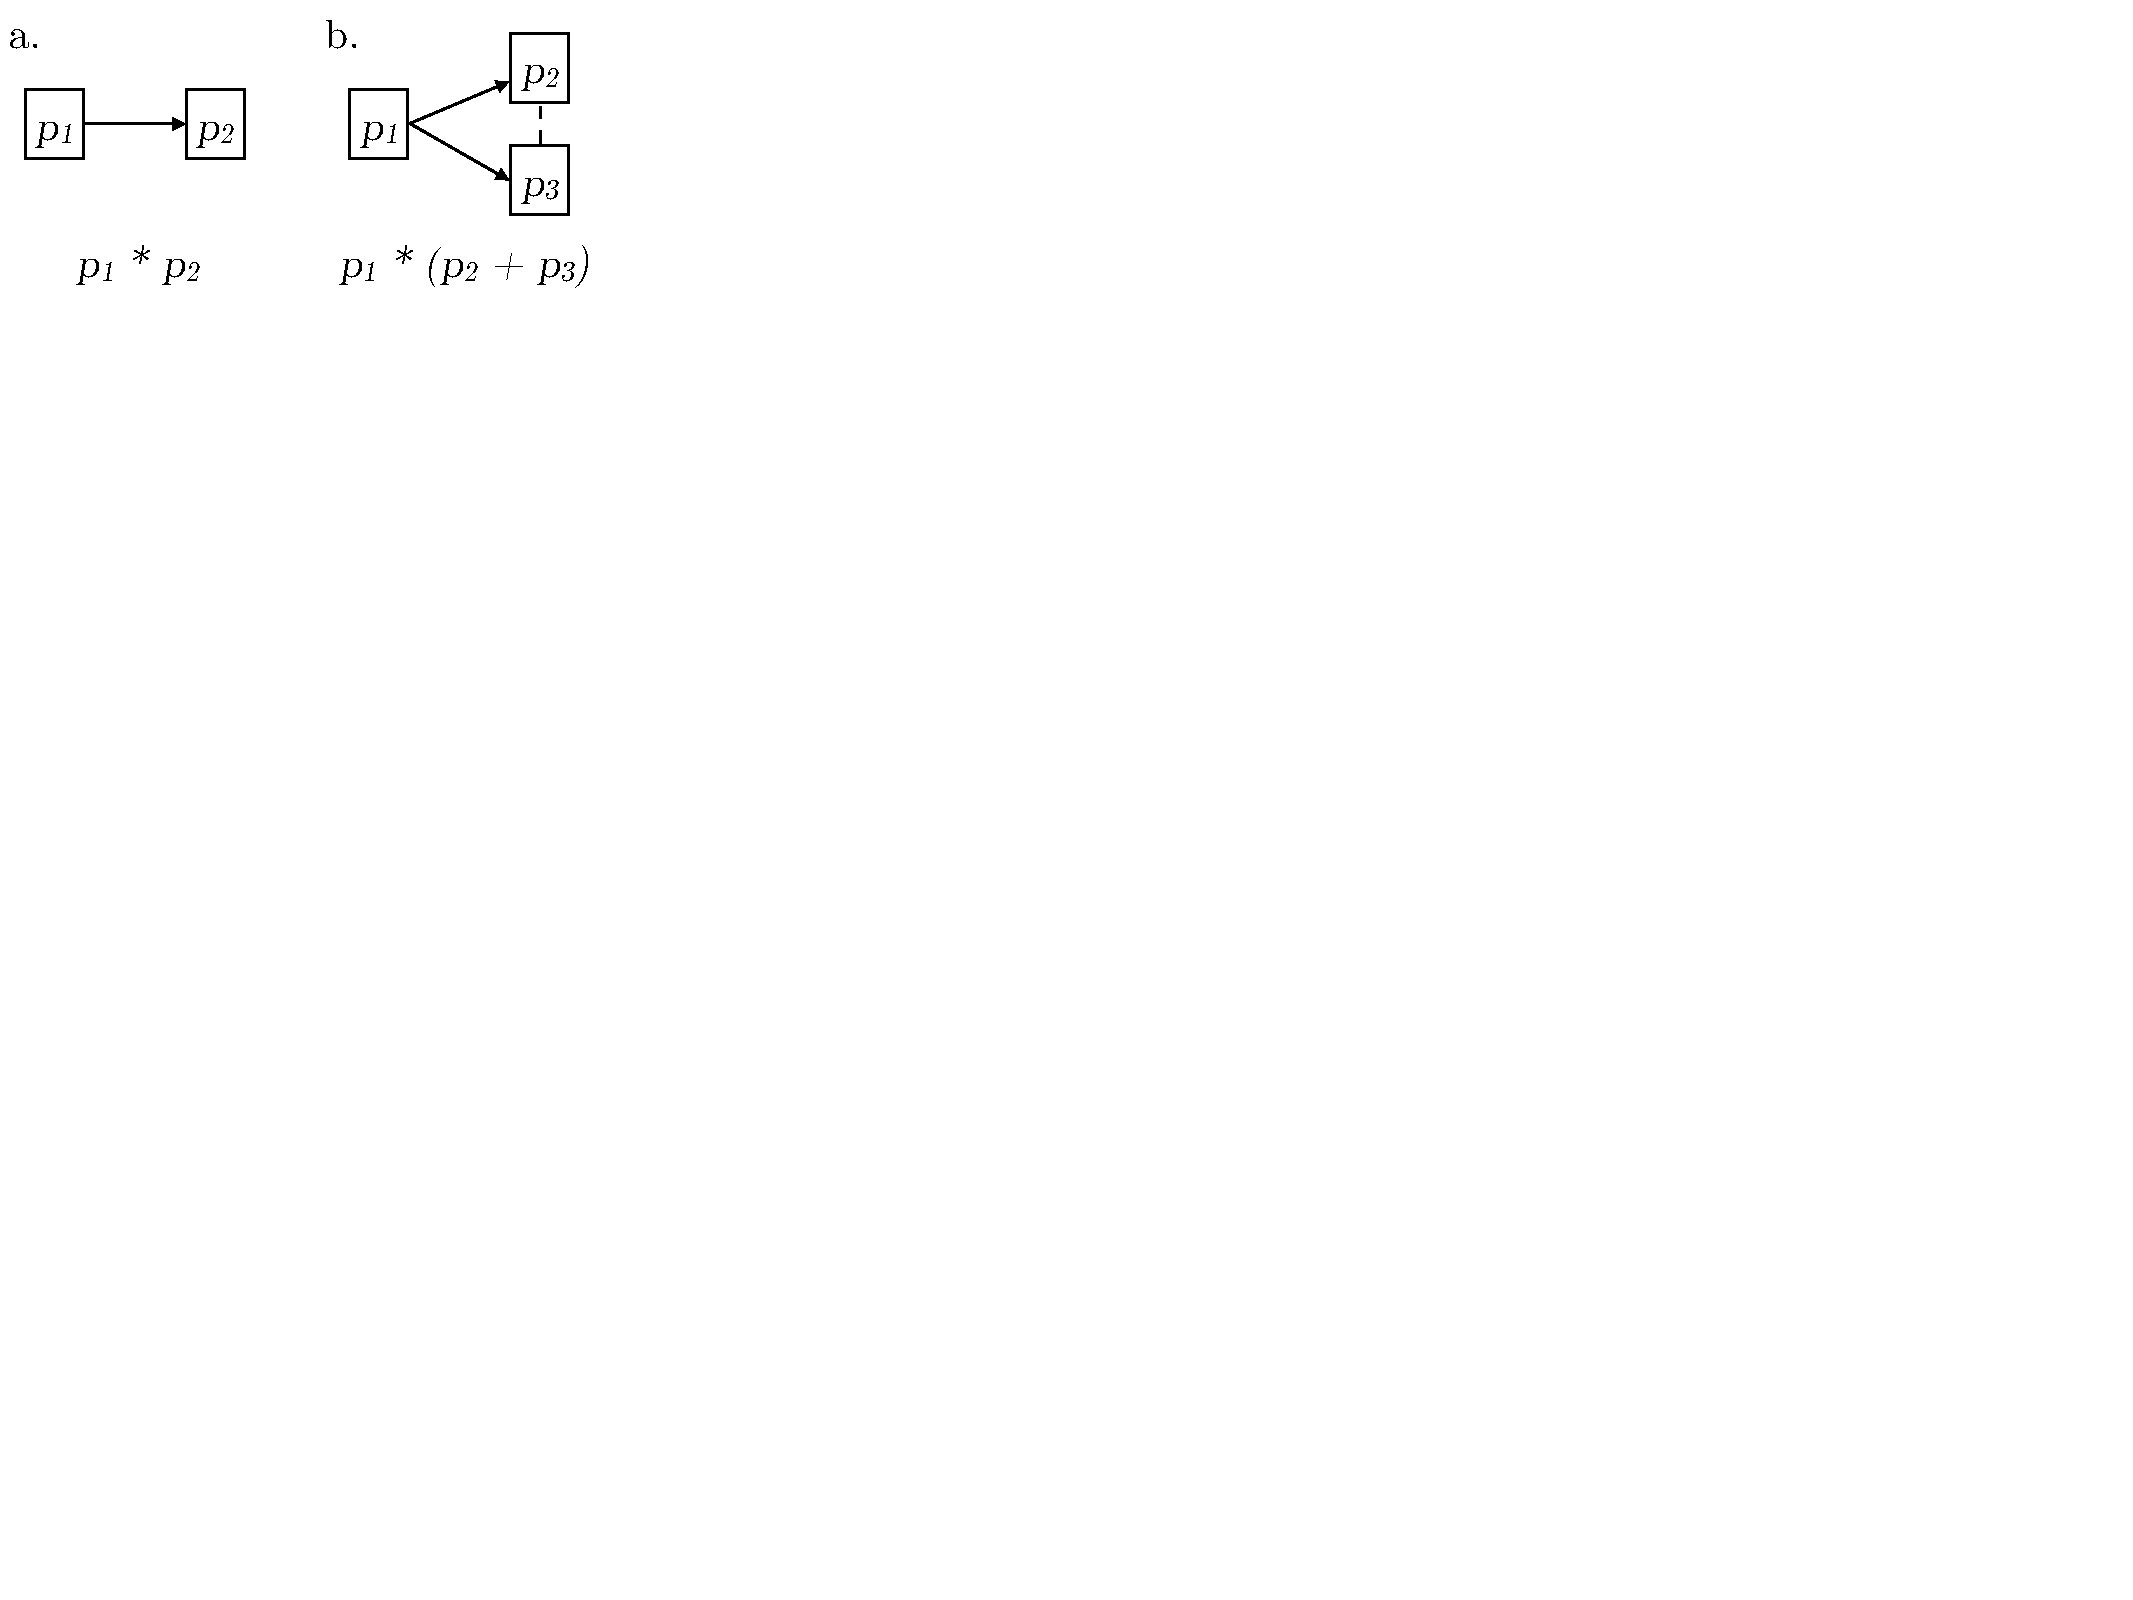
\includegraphics[clip, trim=0in 9.2in 10.25in 0in, width=1.75in]{figures/serial-and-parallel-composition.pdf}
    \vspace{-2mm}
    \caption{a. $p_1$ and $p_2$ composed in serial. b. $p_2$ and $p_3$ composed in parallel.}
    \label{fig:serial-and-parallel-composition}
    \vspace{-2mm}
\end{figure}

\para{The cvs serial composition operator:} Suppose we compose two pipelines $p_1$ and $p_2$ in serial to form the pipeline $p_{12}$, where pipeline $p_i$ has cvs $cvs_i$, inputs $m_{ij} \in M_i$, and where $p_2$'s $w$ bit composition header input is given the special label $c$.

The cvs $cvs_{12}$ contains a cv $cv_{12}$ for each pair of cv $(cv_1, cv_2)$ in $cvs_1$ and $cvs_2$'s cross product. The value of cv $cv_{12}$ for a given subset of inputs $S_{12} \subseteq M_{12}$, where $S_1 = M_1 \cap S_{12}$ and $S_2 = M_2 \cap S_{12}$ is:

\begin{center}
$min[cv_1[S_1] + cv_2[S_2], w + cv_2[S_2], cv_2[S_2, c]]$
\end{center}

\vspace{3mm}
\textit{Proof:} First, we prove that there is a cv $cv_{12}$ for every $(cv_1, cv_2)$ pair. Each cv in a pipeline's cvs represents a path through that pipeline. When $p_1$ and $p_2$ are composed in serial, any path through $p_1$ followed by a path through $p_2$ constitutes a valid path through $p_{12}$ which requires a unique cv.

Next, we prove that the value of $cv_{12}$ for a given $S_{12}$ presented above is correct. Happily, we can prove this very simply by considering $p_{12}$'s paths' dfgs.

Let us label the path that a given $cv_{i}$ measures $path_i$, $path_i$'s dfg $G_i$, and $G_i$'s output node $out_i$. When we compose $path_1$ and $path_2$ to form $path_{12}$, we conceptually link $out_1$ to $path_2$'s composition header $c$. We can therefore build $G_{12}$ from $G_1$ and $G_2$ by adding an edge between $out_1$ and $c$ with capacity $w$ (Figure~\ref{fig:min-cuts-in-composed-pipeline}).

\begin{figure}[tbh]
    \centering
    \vspace{-1mm}
    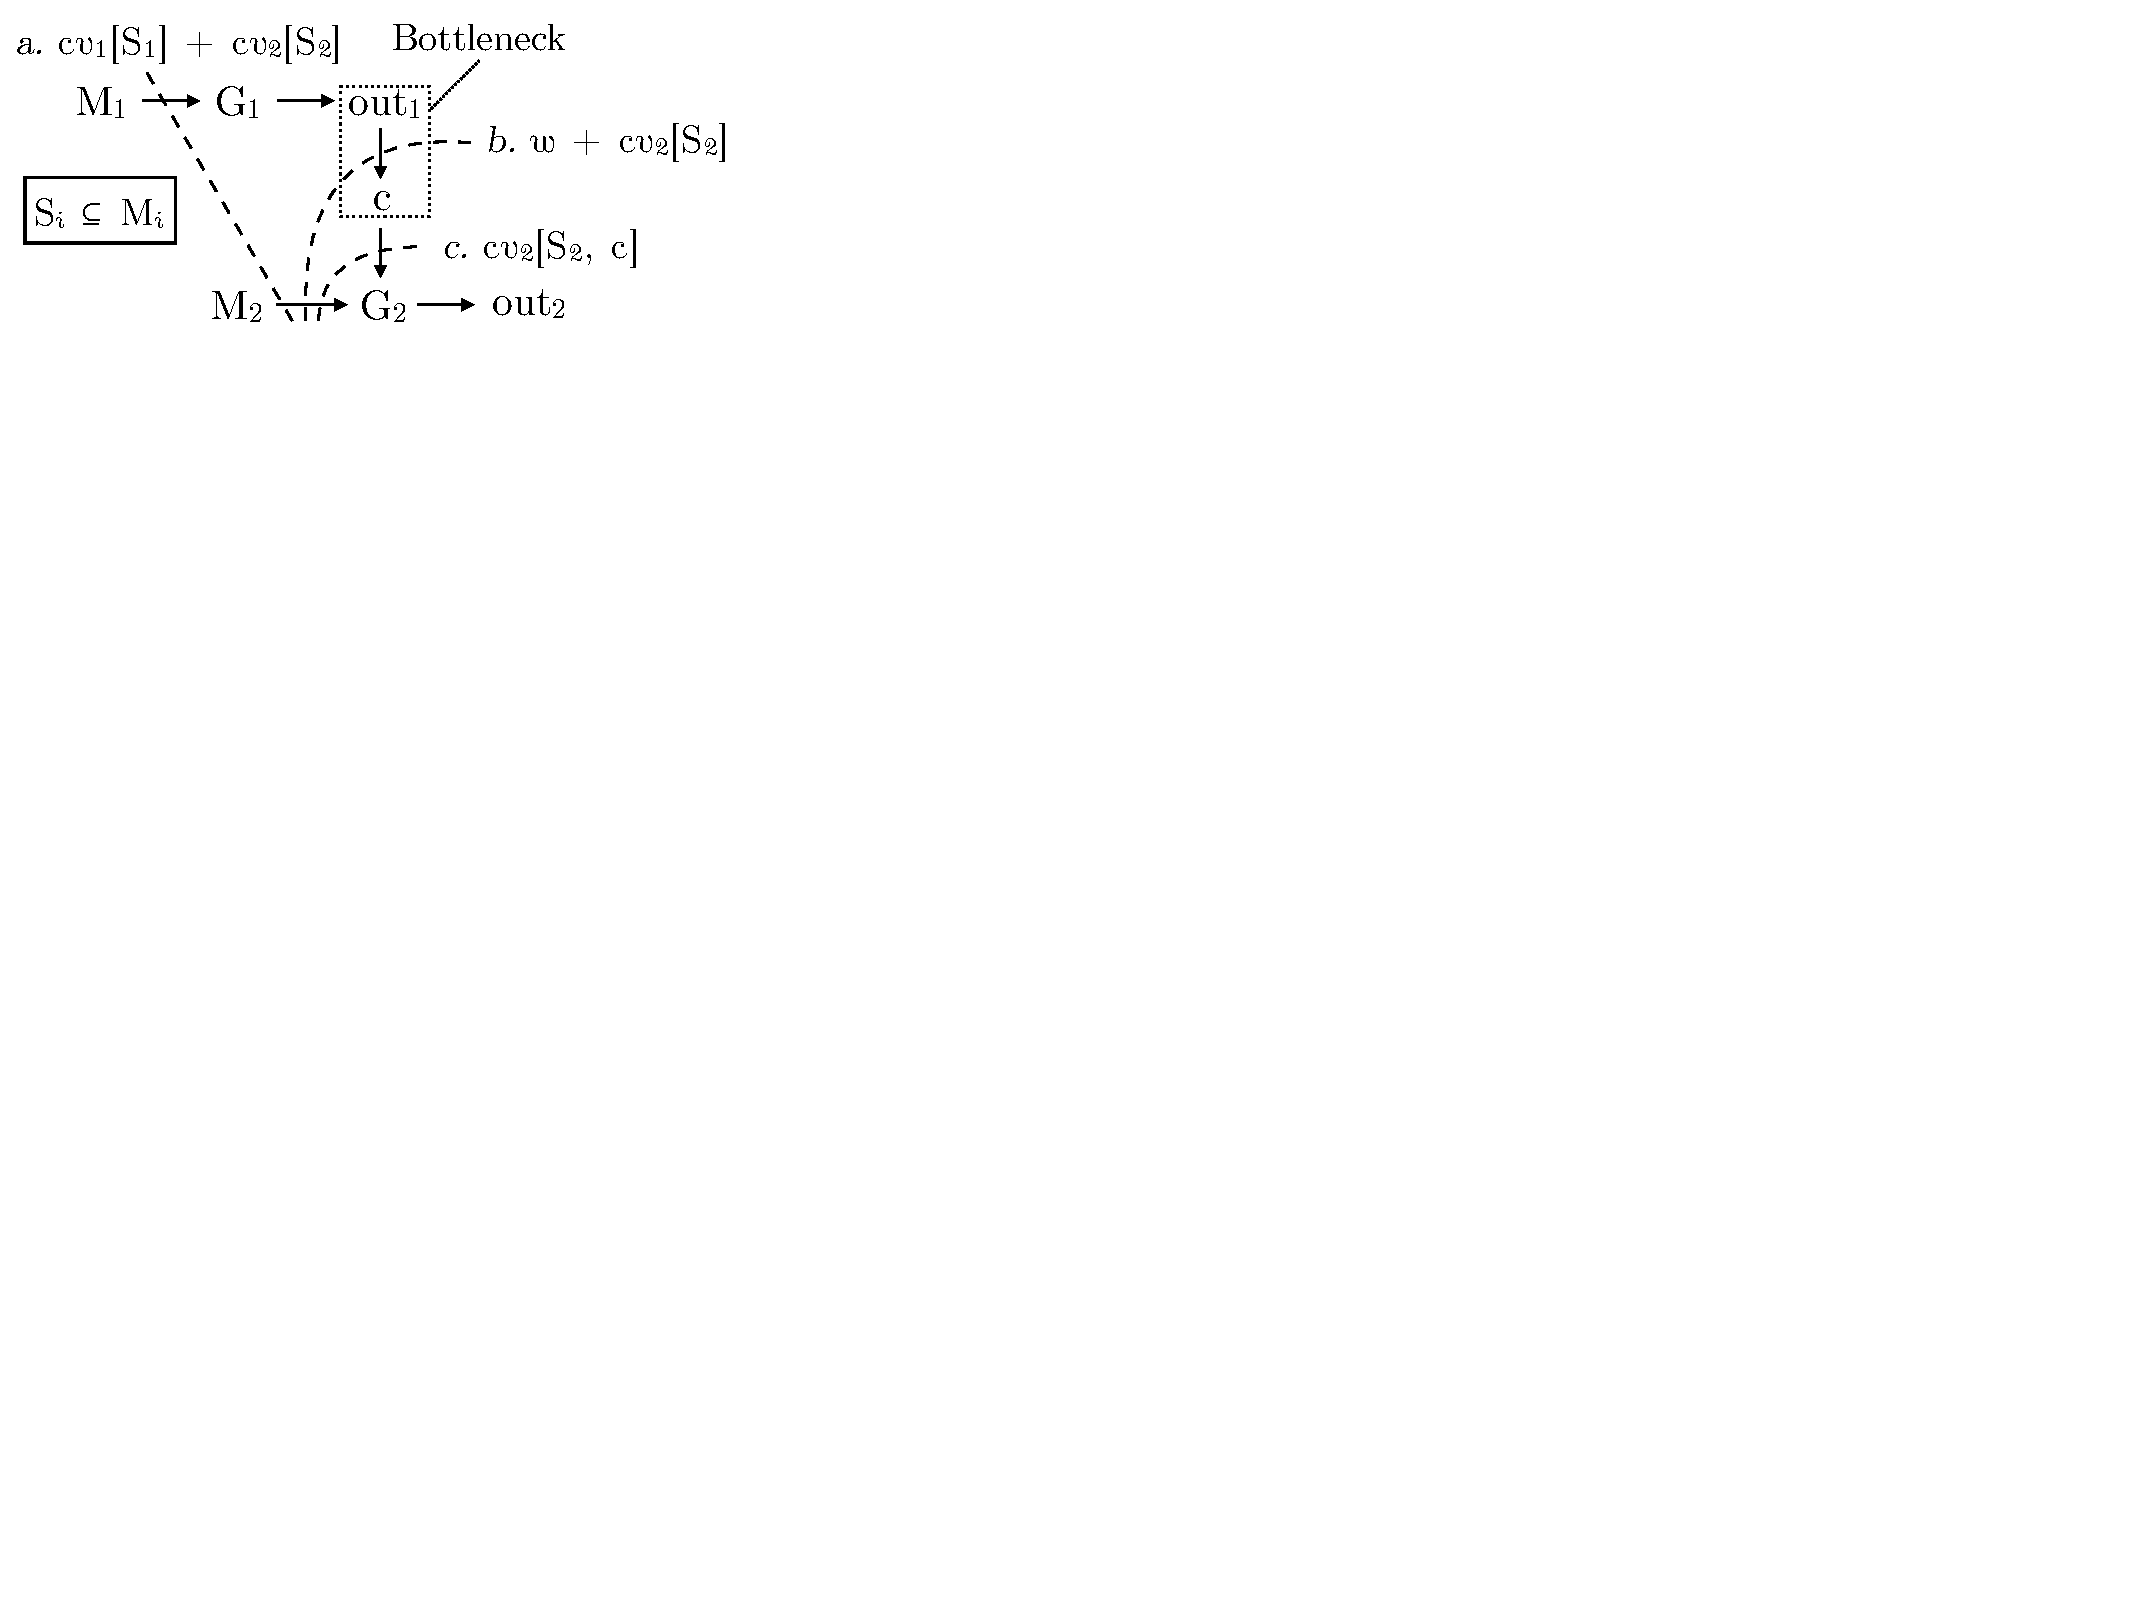
\includegraphics[clip, trim=0in 8.5in 9in 0in, width=2.5in]{figures/min-cuts-in-composed-pipeline.pdf}
    \vspace{-2mm}
    \caption{Min-cuts of $G_{12}$ a. before, b. through and c. after $G_{12}$'s bottleneck and their values.}
    \label{fig:min-cuts-in-composed-pipeline}
    \vspace{-2mm}
\end{figure}


Recall from Section~\ref{sec:pipeline-capacity-theorem} that a given $path_i$'s capacity for a given subset of inputs $cv_i[S_i]$ is the value of the min-cut separating $S_i$ from $out_i$ in $G_i$, and thus that $cv_{12}[S_{12}] = G_{12}.min-cut(S_{12}, out_2)$. The key to finding $S_{12}$'s min-cut is noticing that the edge $(out_1, c)$ forms a bottleneck in $G_{12}$ between $G_1$ and $G_2$, that this min-cut must thus either pass before, through or after this edge, and treating these three cases separately.

\vspace{3mm}
\textit{Case a. min-cut cuts before bottleneck:} The key to finding $S_{12}$'s min-cut in the case that it cuts before $G_{12}$'s bottleneck is noticing that such a min-cut must fully sever $S_1 = S_{12} \cap M_1$ from $out_1$. To see this, consider a min-cut that cuts before $out_1$ which does leave $S_1$ and $out_1$ partially connected. This min-cut must separate $out_1$ from $out_2$, but if $out_1$ and $out_2$ are separated we can decrease the value of the min-cut by leaving every edge between $S_1$ and $out_1$ uncut - a contradiction.

Given the above, in \textit{case a} the min-cut cuts through $G_1$ to sever $S_1$ from $out_1$ and then cuts through $G_2$ to sever any inputs in $S_{12}$ that $G_2$ contains - $S_2$ from $out_2$ (Fig~\ref{fig:min-cuts-in-composed-pipeline}a.) The value of this cut is simply $cv_1[S_1] + cv_2[S_2]$.

\vspace{3mm}
\textit{Case b. min-cut cuts through bottleneck:} In \textit{case b}, the min-cut cuts $(out_1, c)$ to separate $S_1$ from $out_2$, and then cuts through $G_2$ to sever $S_2$ from $out_2$ (Fig~\ref{fig:min-cuts-in-composed-pipeline}b.) The value of this cut is $w + cv_2[S_2]$.

\vspace{3mm}
\textit{Case c. min-cut cuts after bottleneck:} In \textit{case c} the min-cut only cuts $G_2$. To separate $S_1$ from $out_2$, the min-cut must sever both $c$ and $S_2$ from $out_2$. (Fig~\ref{fig:min-cuts-in-composed-pipeline}c.) The value of this cut is $cv_2[c, S_2]$.

\vspace{3mm}
Since the min-cut must either cut before, through or after the bottleneck the min-cut must take one of these three values, and thus we can find $cv_{12}[S_{12}]$ by finding $min[cv_1[S_1] + cv_2[S_2], w + cv_2[S_2], cv_2[S_2, c]]$ as above.

\para{The cvs parallel composition operator:} Suppose we compose two pipelines $p_1$ and $p_2$ in parallel to form the pipeline $p_{12}$, where pipeline $p_i$ has cvs $cvs_i$. $cvs_{12} = cvs_1 \cup cvs_2$

\vspace{3mm}
\textit{Proof:} When $p_1$ and $p_2$ are composed in parallel, incoming packets can take any path through either pipeline and thus every cv in $cv_1$ and $cv_2$ appears in $cv_{12}$.

\para{Pipeline capacity algebra properties:} Now that we have defined our composition operators and their actions on cvs, we show that these operators have certain useful properties: specifically, that they are associative and that $\times$ is distributive over $+$.

\vspace{3mm}
\textit{Distributivity of $\times$ over $+$:} The $\times$ operator can be characterized as a cross-product followed by an element-wise application of our $min[...]$ function, and the $+$ operator can be characterized as a simple union operation. Given these characterizations, $\times$ must be distributive over $+$ because both the cross product operator and any element-wise function are distributive over the union operator.

\vspace{3mm}
\textit{Associativity of $\times$:} Both the cross product of two sets and our $min[...]$ function are associative (proof omitted).

\vspace{3mm}
\textit{Associativity of $+$:} Trivially, the union of two sets is associative.

\subsection{Function transmission vector composition}
In the preceding section, we defined an algebra to calculate the joint cvs of composed pipelines. In this section, we turn our attention to calculating the joint tvs of composed functions. As before, we begin by defining function composition.

\vspace{3mm}
\textsc{Function composition:} Under function composition, one function's output is passed to another as an argument.

\para{Function tvs composition:} We now describe how we calculate the joint tvs of a composed function $f_{cmp}$ from the tvs of an initial function $f_1$ and a mapping from each of $f_1$'s parameters to the function $f_2$, ..., $f_n$, passed as an argument to that parameter (if applicable.)

\cleet{This is precisely the same as serial cvs composition - need to discuss how to merge the two.}